\documentclass{standalone}
\usepackage{amsfonts,amsmath,amssymb}
\usepackage[slovene]{babel}
\usepackage[utf8]{inputenc}
\usepackage[T1]{fontenc}
  
\usepackage{tikz, verbatim}
\usepackage{pgfplots}
\usetikzlibrary{arrows.meta, calc, positioning, automata}

\begin{document}

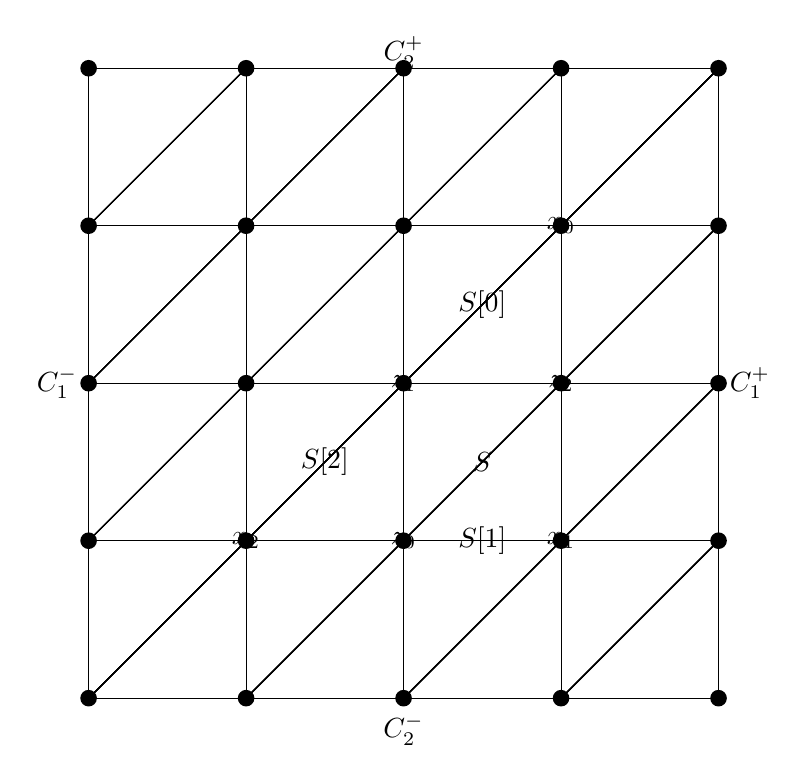
\begin{tikzpicture}
		\foreach \x in {0,2,4,6, 8}
		{   \foreach \y in {0,2,4,6, 8}
		    {  \fill (\x,\y) circle (3pt);
		       \draw (0, \y ) -- (8, \y );
		       \draw (\x ,0) -- (\x ,8);
		       \draw ( 0 , \x) -- ( 8 - \x ,8);
		       \draw ( \x , 0) -- ( 8 ,8 - \x );
		    }
		}	

		
		\draw (-0.4, 4) node {$C_1^-$};
		\draw (8.4, 4) node {$C_1^+$};
		\draw (4, -0.4) node {$C_2^-$};
		\draw (4, 8.2) node {$C_2^+$};	
		\draw (4, 2) node {$z_0$};		
		\draw (4, 4) node {$z_1$};	
		\draw (6, 4) node {$z_2$};	
		\draw (6, 6) node {$x_0$};	
		\draw (6, 2) node {$x_1$};
		\draw (2, 2) node {$x_2$};	
		\draw (5, 3) node {$S$};	
		\draw (5, 5) node {$S[0]$};	
		\draw (5, 2) node {$S[1]$};	
		\draw (3, 3) node {$S[2]$};		
	
	\end{tikzpicture}
	
\end{document}